% Created by tikzDevice version 0.12.3.1 on 2021-05-03 23:03:22
% !TEX encoding = UTF-8 Unicode
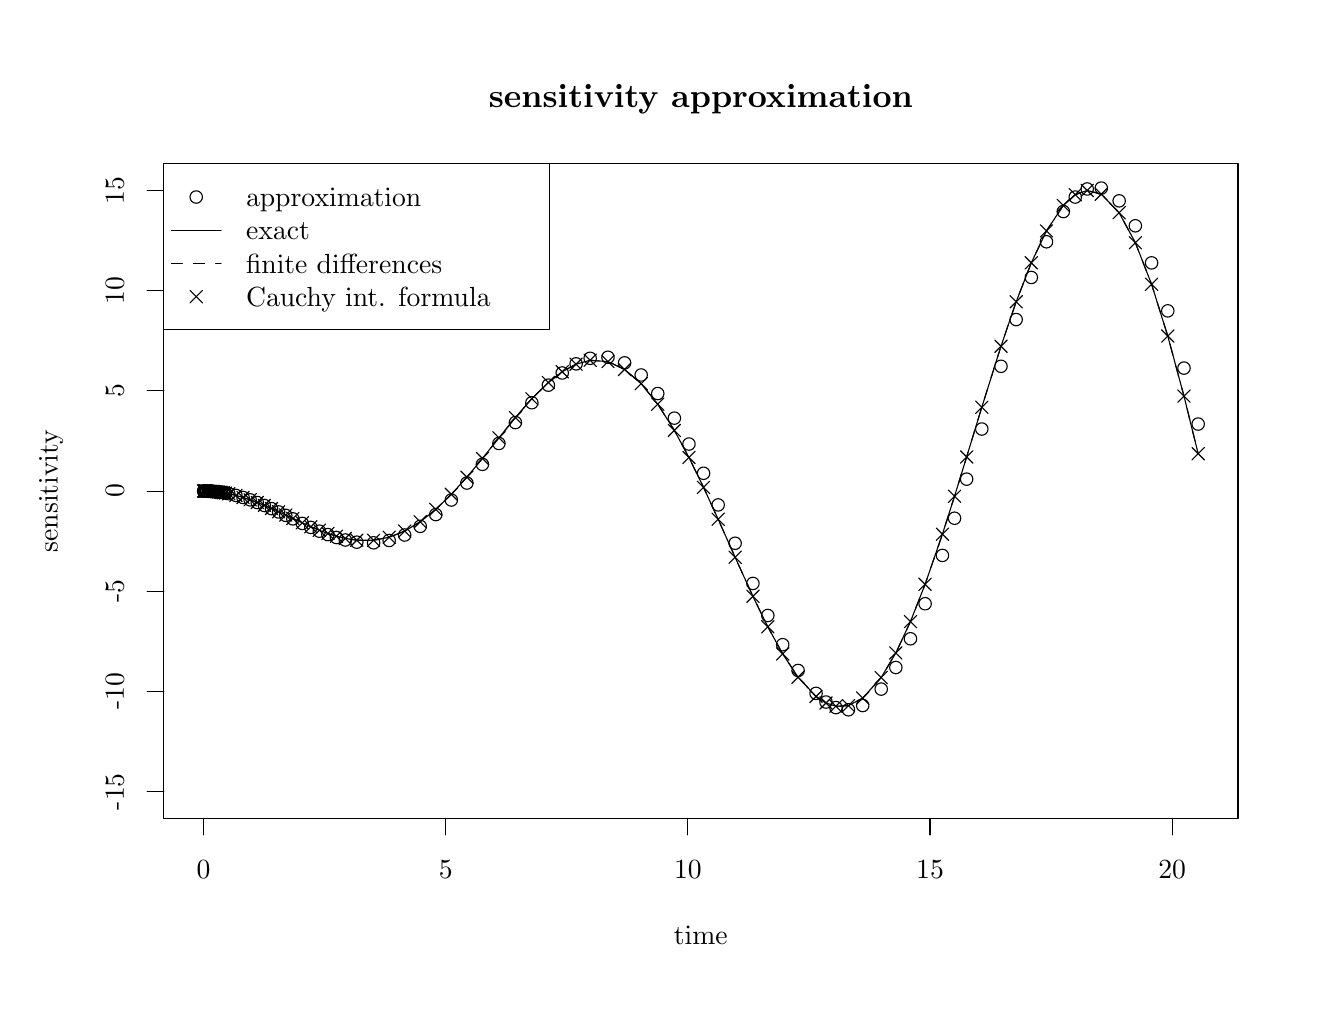
\begin{tikzpicture}[x=1pt,y=1pt]
\definecolor{fillColor}{RGB}{255,255,255}
\path[use as bounding box,fill=fillColor,fill opacity=0.00] (0,0) rectangle (462.53,346.90);
\begin{scope}
\path[clip] ( 49.20, 61.20) rectangle (437.33,297.70);
\definecolor{drawColor}{RGB}{0,0,0}

\path[draw=drawColor,line width= 0.4pt,line join=round,line cap=round] ( 63.58,179.45) circle (  2.25);

\path[draw=drawColor,line width= 0.4pt,line join=round,line cap=round] ( 63.67,179.45) circle (  2.25);

\path[draw=drawColor,line width= 0.4pt,line join=round,line cap=round] ( 63.79,179.45) circle (  2.25);

\path[draw=drawColor,line width= 0.4pt,line join=round,line cap=round] ( 63.91,179.45) circle (  2.25);

\path[draw=drawColor,line width= 0.4pt,line join=round,line cap=round] ( 64.03,179.45) circle (  2.25);

\path[draw=drawColor,line width= 0.4pt,line join=round,line cap=round] ( 64.16,179.44) circle (  2.25);

\path[draw=drawColor,line width= 0.4pt,line join=round,line cap=round] ( 64.28,179.44) circle (  2.25);

\path[draw=drawColor,line width= 0.4pt,line join=round,line cap=round] ( 64.40,179.44) circle (  2.25);

\path[draw=drawColor,line width= 0.4pt,line join=round,line cap=round] ( 64.57,179.44) circle (  2.25);

\path[draw=drawColor,line width= 0.4pt,line join=round,line cap=round] ( 64.84,179.43) circle (  2.25);

\path[draw=drawColor,line width= 0.4pt,line join=round,line cap=round] ( 65.30,179.41) circle (  2.25);

\path[draw=drawColor,line width= 0.4pt,line join=round,line cap=round] ( 65.91,179.38) circle (  2.25);

\path[draw=drawColor,line width= 0.4pt,line join=round,line cap=round] ( 66.51,179.35) circle (  2.25);

\path[draw=drawColor,line width= 0.4pt,line join=round,line cap=round] ( 67.12,179.30) circle (  2.25);

\path[draw=drawColor,line width= 0.4pt,line join=round,line cap=round] ( 67.72,179.25) circle (  2.25);

\path[draw=drawColor,line width= 0.4pt,line join=round,line cap=round] ( 68.33,179.18) circle (  2.25);

\path[draw=drawColor,line width= 0.4pt,line join=round,line cap=round] ( 68.93,179.11) circle (  2.25);

\path[draw=drawColor,line width= 0.4pt,line join=round,line cap=round] ( 69.54,179.03) circle (  2.25);

\path[draw=drawColor,line width= 0.4pt,line join=round,line cap=round] ( 70.14,178.94) circle (  2.25);

\path[draw=drawColor,line width= 0.4pt,line join=round,line cap=round] ( 70.75,178.85) circle (  2.25);

\path[draw=drawColor,line width= 0.4pt,line join=round,line cap=round] ( 71.51,178.71) circle (  2.25);

\path[draw=drawColor,line width= 0.4pt,line join=round,line cap=round] ( 72.67,178.49) circle (  2.25);

\path[draw=drawColor,line width= 0.4pt,line join=round,line cap=round] ( 75.25,177.88) circle (  2.25);

\path[draw=drawColor,line width= 0.4pt,line join=round,line cap=round] ( 77.82,177.14) circle (  2.25);

\path[draw=drawColor,line width= 0.4pt,line join=round,line cap=round] ( 80.39,176.28) circle (  2.25);

\path[draw=drawColor,line width= 0.4pt,line join=round,line cap=round] ( 82.96,175.31) circle (  2.25);

\path[draw=drawColor,line width= 0.4pt,line join=round,line cap=round] ( 85.53,174.24) circle (  2.25);

\path[draw=drawColor,line width= 0.4pt,line join=round,line cap=round] ( 88.11,173.10) circle (  2.25);

\path[draw=drawColor,line width= 0.4pt,line join=round,line cap=round] ( 90.68,171.90) circle (  2.25);

\path[draw=drawColor,line width= 0.4pt,line join=round,line cap=round] ( 93.25,170.67) circle (  2.25);

\path[draw=drawColor,line width= 0.4pt,line join=round,line cap=round] ( 95.82,169.41) circle (  2.25);

\path[draw=drawColor,line width= 0.4pt,line join=round,line cap=round] ( 99.24,167.76) circle (  2.25);

\path[draw=drawColor,line width= 0.4pt,line join=round,line cap=round] (102.32,166.32) circle (  2.25);

\path[draw=drawColor,line width= 0.4pt,line join=round,line cap=round] (105.40,164.96) circle (  2.25);

\path[draw=drawColor,line width= 0.4pt,line join=round,line cap=round] (108.48,163.73) circle (  2.25);

\path[draw=drawColor,line width= 0.4pt,line join=round,line cap=round] (111.55,162.67) circle (  2.25);

\path[draw=drawColor,line width= 0.4pt,line join=round,line cap=round] (114.78,161.77) circle (  2.25);

\path[draw=drawColor,line width= 0.4pt,line join=round,line cap=round] (118.93,160.99) circle (  2.25);

\path[draw=drawColor,line width= 0.4pt,line join=round,line cap=round] (125.00,160.75) circle (  2.25);

\path[draw=drawColor,line width= 0.4pt,line join=round,line cap=round] (130.62,161.60) circle (  2.25);

\path[draw=drawColor,line width= 0.4pt,line join=round,line cap=round] (136.23,163.57) circle (  2.25);

\path[draw=drawColor,line width= 0.4pt,line join=round,line cap=round] (141.85,166.70) circle (  2.25);

\path[draw=drawColor,line width= 0.4pt,line join=round,line cap=round] (147.47,170.95) circle (  2.25);

\path[draw=drawColor,line width= 0.4pt,line join=round,line cap=round] (153.09,176.22) circle (  2.25);

\path[draw=drawColor,line width= 0.4pt,line join=round,line cap=round] (158.71,182.35) circle (  2.25);

\path[draw=drawColor,line width= 0.4pt,line join=round,line cap=round] (164.32,189.11) circle (  2.25);

\path[draw=drawColor,line width= 0.4pt,line join=round,line cap=round] (170.28,196.65) circle (  2.25);

\path[draw=drawColor,line width= 0.4pt,line join=round,line cap=round] (176.24,204.21) circle (  2.25);

\path[draw=drawColor,line width= 0.4pt,line join=round,line cap=round] (182.19,211.37) circle (  2.25);

\path[draw=drawColor,line width= 0.4pt,line join=round,line cap=round] (188.15,217.72) circle (  2.25);

\path[draw=drawColor,line width= 0.4pt,line join=round,line cap=round] (193.16,222.12) circle (  2.25);

\path[draw=drawColor,line width= 0.4pt,line join=round,line cap=round] (198.17,225.42) circle (  2.25);

\path[draw=drawColor,line width= 0.4pt,line join=round,line cap=round] (203.25,227.43) circle (  2.25);

\path[draw=drawColor,line width= 0.4pt,line join=round,line cap=round] (209.69,227.80) circle (  2.25);

\path[draw=drawColor,line width= 0.4pt,line join=round,line cap=round] (215.69,225.78) circle (  2.25);

\path[draw=drawColor,line width= 0.4pt,line join=round,line cap=round] (221.68,221.40) circle (  2.25);

\path[draw=drawColor,line width= 0.4pt,line join=round,line cap=round] (227.68,214.69) circle (  2.25);

\path[draw=drawColor,line width= 0.4pt,line join=round,line cap=round] (233.68,205.81) circle (  2.25);

\path[draw=drawColor,line width= 0.4pt,line join=round,line cap=round] (238.95,196.44) circle (  2.25);

\path[draw=drawColor,line width= 0.4pt,line join=round,line cap=round] (244.23,185.88) circle (  2.25);

\path[draw=drawColor,line width= 0.4pt,line join=round,line cap=round] (249.51,174.45) circle (  2.25);

\path[draw=drawColor,line width= 0.4pt,line join=round,line cap=round] (255.64,160.59) circle (  2.25);

\path[draw=drawColor,line width= 0.4pt,line join=round,line cap=round] (262.06,146.07) circle (  2.25);

\path[draw=drawColor,line width= 0.4pt,line join=round,line cap=round] (267.45,134.49) circle (  2.25);

\path[draw=drawColor,line width= 0.4pt,line join=round,line cap=round] (272.83,123.94) circle (  2.25);

\path[draw=drawColor,line width= 0.4pt,line join=round,line cap=round] (278.39,114.62) circle (  2.25);

\path[draw=drawColor,line width= 0.4pt,line join=round,line cap=round] (284.88,106.36) circle (  2.25);

\path[draw=drawColor,line width= 0.4pt,line join=round,line cap=round] (288.47,103.22) circle (  2.25);

\path[draw=drawColor,line width= 0.4pt,line join=round,line cap=round] (292.05,101.21) circle (  2.25);

\path[draw=drawColor,line width= 0.4pt,line join=round,line cap=round] (296.58,100.42) circle (  2.25);

\path[draw=drawColor,line width= 0.4pt,line join=round,line cap=round] (301.74,101.96) circle (  2.25);

\path[draw=drawColor,line width= 0.4pt,line join=round,line cap=round] (308.42,107.90) circle (  2.25);

\path[draw=drawColor,line width= 0.4pt,line join=round,line cap=round] (313.71,115.70) circle (  2.25);

\path[draw=drawColor,line width= 0.4pt,line join=round,line cap=round] (318.99,126.07) circle (  2.25);

\path[draw=drawColor,line width= 0.4pt,line join=round,line cap=round] (324.28,138.74) circle (  2.25);

\path[draw=drawColor,line width= 0.4pt,line join=round,line cap=round] (330.54,156.20) circle (  2.25);

\path[draw=drawColor,line width= 0.4pt,line join=round,line cap=round] (334.92,169.64) circle (  2.25);

\path[draw=drawColor,line width= 0.4pt,line join=round,line cap=round] (339.29,183.76) circle (  2.25);

\path[draw=drawColor,line width= 0.4pt,line join=round,line cap=round] (344.77,201.87) circle (  2.25);

\path[draw=drawColor,line width= 0.4pt,line join=round,line cap=round] (351.70,224.54) circle (  2.25);

\path[draw=drawColor,line width= 0.4pt,line join=round,line cap=round] (357.18,241.42) circle (  2.25);

\path[draw=drawColor,line width= 0.4pt,line join=round,line cap=round] (362.66,256.63) circle (  2.25);

\path[draw=drawColor,line width= 0.4pt,line join=round,line cap=round] (368.14,269.53) circle (  2.25);

\path[draw=drawColor,line width= 0.4pt,line join=round,line cap=round] (374.23,280.46) circle (  2.25);

\path[draw=drawColor,line width= 0.4pt,line join=round,line cap=round] (378.54,285.69) circle (  2.25);

\path[draw=drawColor,line width= 0.4pt,line join=round,line cap=round] (382.85,288.61) circle (  2.25);

\path[draw=drawColor,line width= 0.4pt,line join=round,line cap=round] (387.95,288.94) circle (  2.25);

\path[draw=drawColor,line width= 0.4pt,line join=round,line cap=round] (394.40,284.32) circle (  2.25);

\path[draw=drawColor,line width= 0.4pt,line join=round,line cap=round] (400.26,275.30) circle (  2.25);

\path[draw=drawColor,line width= 0.4pt,line join=round,line cap=round] (406.12,261.91) circle (  2.25);

\path[draw=drawColor,line width= 0.4pt,line join=round,line cap=round] (411.97,244.57) circle (  2.25);

\path[draw=drawColor,line width= 0.4pt,line join=round,line cap=round] (417.83,223.89) circle (  2.25);

\path[draw=drawColor,line width= 0.4pt,line join=round,line cap=round] (422.95,203.66) circle (  2.25);
\end{scope}
\begin{scope}
\path[clip] (  0.00,  0.00) rectangle (462.53,346.90);
\definecolor{drawColor}{RGB}{0,0,0}

\path[draw=drawColor,line width= 0.4pt,line join=round,line cap=round] ( 63.58, 61.20) -- (413.56, 61.20);

\path[draw=drawColor,line width= 0.4pt,line join=round,line cap=round] ( 63.58, 61.20) -- ( 63.58, 55.20);

\path[draw=drawColor,line width= 0.4pt,line join=round,line cap=round] (151.07, 61.20) -- (151.07, 55.20);

\path[draw=drawColor,line width= 0.4pt,line join=round,line cap=round] (238.57, 61.20) -- (238.57, 55.20);

\path[draw=drawColor,line width= 0.4pt,line join=round,line cap=round] (326.07, 61.20) -- (326.07, 55.20);

\path[draw=drawColor,line width= 0.4pt,line join=round,line cap=round] (413.56, 61.20) -- (413.56, 55.20);

\node[text=drawColor,anchor=base,inner sep=0pt, outer sep=0pt, scale=  1.00] at ( 63.58, 39.60) {0};

\node[text=drawColor,anchor=base,inner sep=0pt, outer sep=0pt, scale=  1.00] at (151.07, 39.60) {5};

\node[text=drawColor,anchor=base,inner sep=0pt, outer sep=0pt, scale=  1.00] at (238.57, 39.60) {10};

\node[text=drawColor,anchor=base,inner sep=0pt, outer sep=0pt, scale=  1.00] at (326.07, 39.60) {15};

\node[text=drawColor,anchor=base,inner sep=0pt, outer sep=0pt, scale=  1.00] at (413.56, 39.60) {20};

\path[draw=drawColor,line width= 0.4pt,line join=round,line cap=round] ( 49.20, 70.83) -- ( 49.20,288.06);

\path[draw=drawColor,line width= 0.4pt,line join=round,line cap=round] ( 49.20, 70.83) -- ( 43.20, 70.83);

\path[draw=drawColor,line width= 0.4pt,line join=round,line cap=round] ( 49.20,107.04) -- ( 43.20,107.04);

\path[draw=drawColor,line width= 0.4pt,line join=round,line cap=round] ( 49.20,143.24) -- ( 43.20,143.24);

\path[draw=drawColor,line width= 0.4pt,line join=round,line cap=round] ( 49.20,179.45) -- ( 43.20,179.45);

\path[draw=drawColor,line width= 0.4pt,line join=round,line cap=round] ( 49.20,215.65) -- ( 43.20,215.65);

\path[draw=drawColor,line width= 0.4pt,line join=round,line cap=round] ( 49.20,251.86) -- ( 43.20,251.86);

\path[draw=drawColor,line width= 0.4pt,line join=round,line cap=round] ( 49.20,288.06) -- ( 43.20,288.06);

\node[text=drawColor,rotate= 90.00,anchor=base,inner sep=0pt, outer sep=0pt, scale=  1.00] at ( 34.80, 70.83) {-15};

\node[text=drawColor,rotate= 90.00,anchor=base,inner sep=0pt, outer sep=0pt, scale=  1.00] at ( 34.80,107.04) {-10};

\node[text=drawColor,rotate= 90.00,anchor=base,inner sep=0pt, outer sep=0pt, scale=  1.00] at ( 34.80,143.24) {-5};

\node[text=drawColor,rotate= 90.00,anchor=base,inner sep=0pt, outer sep=0pt, scale=  1.00] at ( 34.80,179.45) {0};

\node[text=drawColor,rotate= 90.00,anchor=base,inner sep=0pt, outer sep=0pt, scale=  1.00] at ( 34.80,215.65) {5};

\node[text=drawColor,rotate= 90.00,anchor=base,inner sep=0pt, outer sep=0pt, scale=  1.00] at ( 34.80,251.86) {10};

\node[text=drawColor,rotate= 90.00,anchor=base,inner sep=0pt, outer sep=0pt, scale=  1.00] at ( 34.80,288.06) {15};

\path[draw=drawColor,line width= 0.4pt,line join=round,line cap=round] ( 49.20, 61.20) --
	(437.33, 61.20) --
	(437.33,297.70) --
	( 49.20,297.70) --
	( 49.20, 61.20);
\end{scope}
\begin{scope}
\path[clip] (  0.00,  0.00) rectangle (462.53,346.90);
\definecolor{drawColor}{RGB}{0,0,0}

\node[text=drawColor,anchor=base,inner sep=0pt, outer sep=0pt, scale=  1.20] at (243.26,318.16) {\bfseries sensitivity approximation};

\node[text=drawColor,anchor=base,inner sep=0pt, outer sep=0pt, scale=  1.00] at (243.26, 15.60) {time};

\node[text=drawColor,rotate= 90.00,anchor=base,inner sep=0pt, outer sep=0pt, scale=  1.00] at ( 10.80,179.45) {sensitivity};
\end{scope}
\begin{scope}
\path[clip] ( 49.20, 61.20) rectangle (437.33,297.70);
\definecolor{drawColor}{RGB}{0,0,0}

\path[draw=drawColor,line width= 0.4pt,line join=round,line cap=round] ( 63.58,179.45) --
	( 63.67,179.45) --
	( 63.79,179.45) --
	( 63.91,179.45) --
	( 64.03,179.45) --
	( 64.16,179.44) --
	( 64.28,179.44) --
	( 64.40,179.44) --
	( 64.57,179.44) --
	( 64.84,179.43) --
	( 65.30,179.41) --
	( 65.91,179.38) --
	( 66.51,179.35) --
	( 67.12,179.30) --
	( 67.72,179.25) --
	( 68.33,179.18) --
	( 68.93,179.11) --
	( 69.54,179.03) --
	( 70.14,178.94) --
	( 70.75,178.85) --
	( 71.51,178.71) --
	( 72.67,178.49) --
	( 75.25,177.88) --
	( 77.82,177.15) --
	( 80.39,176.29) --
	( 82.96,175.33) --
	( 85.53,174.28) --
	( 88.11,173.16) --
	( 90.68,171.99) --
	( 93.25,170.78) --
	( 95.82,169.56) --
	( 99.24,167.96) --
	(102.32,166.57) --
	(105.40,165.29) --
	(108.48,164.13) --
	(111.55,163.15) --
	(114.78,162.34) --
	(118.93,161.70) --
	(125.00,161.68) --
	(130.62,162.76) --
	(136.23,164.98) --
	(141.85,168.35) --
	(147.47,172.82) --
	(153.09,178.26) --
	(158.71,184.48) --
	(164.32,191.24) --
	(170.28,198.68) --
	(176.24,206.01) --
	(182.19,212.82) --
	(188.15,218.68) --
	(193.16,222.58) --
	(198.17,225.31) --
	(203.25,226.70) --
	(209.69,226.23) --
	(215.69,223.41) --
	(221.68,218.25) --
	(227.68,210.84) --
	(233.68,201.37) --
	(238.95,191.60) --
	(244.23,180.78) --
	(249.51,169.26) --
	(255.64,155.52) --
	(262.06,141.42) --
	(267.45,130.39) --
	(272.83,120.58) --
	(278.39,112.20) --
	(284.88,105.23) --
	(288.47,102.87) --
	(292.05,101.68) --
	(296.58,101.92) --
	(301.74,104.64) --
	(308.42,112.08) --
	(313.71,120.96) --
	(318.99,132.29) --
	(324.28,145.75) --
	(330.54,163.88) --
	(334.92,177.58) --
	(339.29,191.79) --
	(344.77,209.74) --
	(351.70,231.78) --
	(357.18,247.82) --
	(362.66,261.92) --
	(368.14,273.47) --
	(374.23,282.67) --
	(378.54,286.55) --
	(382.85,288.08) --
	(387.95,286.73) --
	(394.40,280.01) --
	(400.26,269.19) --
	(406.12,254.18) --
	(411.97,235.48) --
	(417.83,213.76) --
	(422.95,192.95);

\path[draw=drawColor,line width= 0.4pt,dash pattern=on 4pt off 4pt ,line join=round,line cap=round] ( 63.58,179.45) --
	( 63.67,179.45) --
	( 63.79,179.45) --
	( 63.91,179.45) --
	( 64.03,179.45) --
	( 64.16,179.44) --
	( 64.28,179.44) --
	( 64.40,179.44) --
	( 64.57,179.44) --
	( 64.84,179.43) --
	( 65.30,179.41) --
	( 65.91,179.38) --
	( 66.51,179.35) --
	( 67.12,179.30) --
	( 67.72,179.25) --
	( 68.33,179.18) --
	( 68.93,179.11) --
	( 69.54,179.03) --
	( 70.14,178.94) --
	( 70.75,178.85) --
	( 71.51,178.71) --
	( 72.67,178.49) --
	( 75.25,177.88) --
	( 77.82,177.15) --
	( 80.39,176.29) --
	( 82.96,175.33) --
	( 85.53,174.28) --
	( 88.11,173.16) --
	( 90.68,171.99) --
	( 93.25,170.78) --
	( 95.82,169.56) --
	( 99.24,167.96) --
	(102.32,166.57) --
	(105.40,165.29) --
	(108.48,164.13) --
	(111.55,163.15) --
	(114.78,162.34) --
	(118.93,161.70) --
	(125.00,161.68) --
	(130.62,162.76) --
	(136.23,164.98) --
	(141.85,168.35) --
	(147.47,172.82) --
	(153.09,178.26) --
	(158.71,184.48) --
	(164.32,191.24) --
	(170.28,198.68) --
	(176.24,206.01) --
	(182.19,212.82) --
	(188.15,218.68) --
	(193.16,222.58) --
	(198.17,225.31) --
	(203.25,226.70) --
	(209.69,226.23) --
	(215.69,223.41) --
	(221.68,218.25) --
	(227.68,210.84) --
	(233.68,201.37) --
	(238.95,191.60) --
	(244.23,180.78) --
	(249.51,169.26) --
	(255.64,155.52) --
	(262.06,141.42) --
	(267.45,130.39) --
	(272.83,120.58) --
	(278.39,112.20) --
	(284.88,105.23) --
	(288.47,102.87) --
	(292.05,101.68) --
	(296.58,101.92) --
	(301.74,104.64) --
	(308.42,112.08) --
	(313.71,120.96) --
	(318.99,132.29) --
	(324.28,145.75) --
	(330.54,163.88) --
	(334.92,177.58) --
	(339.29,191.79) --
	(344.77,209.74) --
	(351.70,231.78) --
	(357.18,247.82) --
	(362.66,261.92) --
	(368.14,273.47) --
	(374.23,282.67) --
	(378.54,286.55) --
	(382.85,288.08) --
	(387.95,286.73) --
	(394.40,280.01) --
	(400.26,269.19) --
	(406.12,254.18) --
	(411.97,235.48) --
	(417.83,213.76) --
	(422.95,192.95);

\path[draw=drawColor,line width= 0.4pt,line join=round,line cap=round] ( 61.33,177.20) -- ( 65.83,181.70);

\path[draw=drawColor,line width= 0.4pt,line join=round,line cap=round] ( 61.33,181.70) -- ( 65.83,177.20);

\path[draw=drawColor,line width= 0.4pt,line join=round,line cap=round] ( 61.42,177.20) -- ( 65.92,181.70);

\path[draw=drawColor,line width= 0.4pt,line join=round,line cap=round] ( 61.42,181.70) -- ( 65.92,177.20);

\path[draw=drawColor,line width= 0.4pt,line join=round,line cap=round] ( 61.54,177.20) -- ( 66.04,181.70);

\path[draw=drawColor,line width= 0.4pt,line join=round,line cap=round] ( 61.54,181.70) -- ( 66.04,177.20);

\path[draw=drawColor,line width= 0.4pt,line join=round,line cap=round] ( 61.66,177.20) -- ( 66.16,181.70);

\path[draw=drawColor,line width= 0.4pt,line join=round,line cap=round] ( 61.66,181.70) -- ( 66.16,177.20);

\path[draw=drawColor,line width= 0.4pt,line join=round,line cap=round] ( 61.78,177.20) -- ( 66.28,181.70);

\path[draw=drawColor,line width= 0.4pt,line join=round,line cap=round] ( 61.78,181.70) -- ( 66.28,177.20);

\path[draw=drawColor,line width= 0.4pt,line join=round,line cap=round] ( 61.91,177.19) -- ( 66.41,181.69);

\path[draw=drawColor,line width= 0.4pt,line join=round,line cap=round] ( 61.91,181.69) -- ( 66.41,177.19);

\path[draw=drawColor,line width= 0.4pt,line join=round,line cap=round] ( 62.03,177.19) -- ( 66.53,181.69);

\path[draw=drawColor,line width= 0.4pt,line join=round,line cap=round] ( 62.03,181.69) -- ( 66.53,177.19);

\path[draw=drawColor,line width= 0.4pt,line join=round,line cap=round] ( 62.15,177.19) -- ( 66.65,181.69);

\path[draw=drawColor,line width= 0.4pt,line join=round,line cap=round] ( 62.15,181.69) -- ( 66.65,177.19);

\path[draw=drawColor,line width= 0.4pt,line join=round,line cap=round] ( 62.32,177.19) -- ( 66.82,181.69);

\path[draw=drawColor,line width= 0.4pt,line join=round,line cap=round] ( 62.32,181.69) -- ( 66.82,177.19);

\path[draw=drawColor,line width= 0.4pt,line join=round,line cap=round] ( 62.59,177.18) -- ( 67.09,181.68);

\path[draw=drawColor,line width= 0.4pt,line join=round,line cap=round] ( 62.59,181.68) -- ( 67.09,177.18);

\path[draw=drawColor,line width= 0.4pt,line join=round,line cap=round] ( 63.05,177.16) -- ( 67.55,181.66);

\path[draw=drawColor,line width= 0.4pt,line join=round,line cap=round] ( 63.05,181.66) -- ( 67.55,177.16);

\path[draw=drawColor,line width= 0.4pt,line join=round,line cap=round] ( 63.66,177.13) -- ( 68.16,181.63);

\path[draw=drawColor,line width= 0.4pt,line join=round,line cap=round] ( 63.66,181.63) -- ( 68.16,177.13);

\path[draw=drawColor,line width= 0.4pt,line join=round,line cap=round] ( 64.26,177.10) -- ( 68.76,181.60);

\path[draw=drawColor,line width= 0.4pt,line join=round,line cap=round] ( 64.26,181.60) -- ( 68.76,177.10);

\path[draw=drawColor,line width= 0.4pt,line join=round,line cap=round] ( 64.87,177.05) -- ( 69.37,181.55);

\path[draw=drawColor,line width= 0.4pt,line join=round,line cap=round] ( 64.87,181.55) -- ( 69.37,177.05);

\path[draw=drawColor,line width= 0.4pt,line join=round,line cap=round] ( 65.47,177.00) -- ( 69.97,181.50);

\path[draw=drawColor,line width= 0.4pt,line join=round,line cap=round] ( 65.47,181.50) -- ( 69.97,177.00);

\path[draw=drawColor,line width= 0.4pt,line join=round,line cap=round] ( 66.08,176.93) -- ( 70.58,181.43);

\path[draw=drawColor,line width= 0.4pt,line join=round,line cap=round] ( 66.08,181.43) -- ( 70.58,176.93);

\path[draw=drawColor,line width= 0.4pt,line join=round,line cap=round] ( 66.68,176.86) -- ( 71.18,181.36);

\path[draw=drawColor,line width= 0.4pt,line join=round,line cap=round] ( 66.68,181.36) -- ( 71.18,176.86);

\path[draw=drawColor,line width= 0.4pt,line join=round,line cap=round] ( 67.29,176.78) -- ( 71.79,181.28);

\path[draw=drawColor,line width= 0.4pt,line join=round,line cap=round] ( 67.29,181.28) -- ( 71.79,176.78);

\path[draw=drawColor,line width= 0.4pt,line join=round,line cap=round] ( 67.89,176.69) -- ( 72.39,181.19);

\path[draw=drawColor,line width= 0.4pt,line join=round,line cap=round] ( 67.89,181.19) -- ( 72.39,176.69);

\path[draw=drawColor,line width= 0.4pt,line join=round,line cap=round] ( 68.50,176.60) -- ( 73.00,181.10);

\path[draw=drawColor,line width= 0.4pt,line join=round,line cap=round] ( 68.50,181.10) -- ( 73.00,176.60);

\path[draw=drawColor,line width= 0.4pt,line join=round,line cap=round] ( 69.26,176.46) -- ( 73.76,180.96);

\path[draw=drawColor,line width= 0.4pt,line join=round,line cap=round] ( 69.26,180.96) -- ( 73.76,176.46);

\path[draw=drawColor,line width= 0.4pt,line join=round,line cap=round] ( 70.42,176.24) -- ( 74.92,180.74);

\path[draw=drawColor,line width= 0.4pt,line join=round,line cap=round] ( 70.42,180.74) -- ( 74.92,176.24);

\path[draw=drawColor,line width= 0.4pt,line join=round,line cap=round] ( 73.00,175.63) -- ( 77.50,180.13);

\path[draw=drawColor,line width= 0.4pt,line join=round,line cap=round] ( 73.00,180.13) -- ( 77.50,175.63);

\path[draw=drawColor,line width= 0.4pt,line join=round,line cap=round] ( 75.57,174.90) -- ( 80.07,179.40);

\path[draw=drawColor,line width= 0.4pt,line join=round,line cap=round] ( 75.57,179.40) -- ( 80.07,174.90);

\path[draw=drawColor,line width= 0.4pt,line join=round,line cap=round] ( 78.14,174.04) -- ( 82.64,178.54);

\path[draw=drawColor,line width= 0.4pt,line join=round,line cap=round] ( 78.14,178.54) -- ( 82.64,174.04);

\path[draw=drawColor,line width= 0.4pt,line join=round,line cap=round] ( 80.71,173.08) -- ( 85.21,177.58);

\path[draw=drawColor,line width= 0.4pt,line join=round,line cap=round] ( 80.71,177.58) -- ( 85.21,173.08);

\path[draw=drawColor,line width= 0.4pt,line join=round,line cap=round] ( 83.28,172.03) -- ( 87.78,176.53);

\path[draw=drawColor,line width= 0.4pt,line join=round,line cap=round] ( 83.28,176.53) -- ( 87.78,172.03);

\path[draw=drawColor,line width= 0.4pt,line join=round,line cap=round] ( 85.86,170.91) -- ( 90.36,175.41);

\path[draw=drawColor,line width= 0.4pt,line join=round,line cap=round] ( 85.86,175.41) -- ( 90.36,170.91);

\path[draw=drawColor,line width= 0.4pt,line join=round,line cap=round] ( 88.43,169.74) -- ( 92.93,174.24);

\path[draw=drawColor,line width= 0.4pt,line join=round,line cap=round] ( 88.43,174.24) -- ( 92.93,169.74);

\path[draw=drawColor,line width= 0.4pt,line join=round,line cap=round] ( 91.00,168.53) -- ( 95.50,173.03);

\path[draw=drawColor,line width= 0.4pt,line join=round,line cap=round] ( 91.00,173.03) -- ( 95.50,168.53);

\path[draw=drawColor,line width= 0.4pt,line join=round,line cap=round] ( 93.57,167.31) -- ( 98.07,171.81);

\path[draw=drawColor,line width= 0.4pt,line join=round,line cap=round] ( 93.57,171.81) -- ( 98.07,167.31);

\path[draw=drawColor,line width= 0.4pt,line join=round,line cap=round] ( 96.99,165.71) -- (101.49,170.21);

\path[draw=drawColor,line width= 0.4pt,line join=round,line cap=round] ( 96.99,170.21) -- (101.49,165.71);

\path[draw=drawColor,line width= 0.4pt,line join=round,line cap=round] (100.07,164.32) -- (104.57,168.82);

\path[draw=drawColor,line width= 0.4pt,line join=round,line cap=round] (100.07,168.82) -- (104.57,164.32);

\path[draw=drawColor,line width= 0.4pt,line join=round,line cap=round] (103.15,163.04) -- (107.65,167.54);

\path[draw=drawColor,line width= 0.4pt,line join=round,line cap=round] (103.15,167.54) -- (107.65,163.04);

\path[draw=drawColor,line width= 0.4pt,line join=round,line cap=round] (106.23,161.88) -- (110.73,166.38);

\path[draw=drawColor,line width= 0.4pt,line join=round,line cap=round] (106.23,166.38) -- (110.73,161.88);

\path[draw=drawColor,line width= 0.4pt,line join=round,line cap=round] (109.30,160.90) -- (113.80,165.40);

\path[draw=drawColor,line width= 0.4pt,line join=round,line cap=round] (109.30,165.40) -- (113.80,160.90);

\path[draw=drawColor,line width= 0.4pt,line join=round,line cap=round] (112.53,160.09) -- (117.03,164.59);

\path[draw=drawColor,line width= 0.4pt,line join=round,line cap=round] (112.53,164.59) -- (117.03,160.09);

\path[draw=drawColor,line width= 0.4pt,line join=round,line cap=round] (116.68,159.45) -- (121.18,163.95);

\path[draw=drawColor,line width= 0.4pt,line join=round,line cap=round] (116.68,163.95) -- (121.18,159.45);

\path[draw=drawColor,line width= 0.4pt,line join=round,line cap=round] (122.75,159.43) -- (127.25,163.93);

\path[draw=drawColor,line width= 0.4pt,line join=round,line cap=round] (122.75,163.93) -- (127.25,159.43);

\path[draw=drawColor,line width= 0.4pt,line join=round,line cap=round] (128.37,160.51) -- (132.87,165.01);

\path[draw=drawColor,line width= 0.4pt,line join=round,line cap=round] (128.37,165.01) -- (132.87,160.51);

\path[draw=drawColor,line width= 0.4pt,line join=round,line cap=round] (133.98,162.73) -- (138.48,167.23);

\path[draw=drawColor,line width= 0.4pt,line join=round,line cap=round] (133.98,167.23) -- (138.48,162.73);

\path[draw=drawColor,line width= 0.4pt,line join=round,line cap=round] (139.60,166.10) -- (144.10,170.60);

\path[draw=drawColor,line width= 0.4pt,line join=round,line cap=round] (139.60,170.60) -- (144.10,166.10);

\path[draw=drawColor,line width= 0.4pt,line join=round,line cap=round] (145.22,170.57) -- (149.72,175.07);

\path[draw=drawColor,line width= 0.4pt,line join=round,line cap=round] (145.22,175.07) -- (149.72,170.57);

\path[draw=drawColor,line width= 0.4pt,line join=round,line cap=round] (150.84,176.01) -- (155.34,180.51);

\path[draw=drawColor,line width= 0.4pt,line join=round,line cap=round] (150.84,180.51) -- (155.34,176.01);

\path[draw=drawColor,line width= 0.4pt,line join=round,line cap=round] (156.46,182.23) -- (160.96,186.73);

\path[draw=drawColor,line width= 0.4pt,line join=round,line cap=round] (156.46,186.73) -- (160.96,182.23);

\path[draw=drawColor,line width= 0.4pt,line join=round,line cap=round] (162.07,188.99) -- (166.57,193.49);

\path[draw=drawColor,line width= 0.4pt,line join=round,line cap=round] (162.07,193.49) -- (166.57,188.99);

\path[draw=drawColor,line width= 0.4pt,line join=round,line cap=round] (168.03,196.43) -- (172.53,200.93);

\path[draw=drawColor,line width= 0.4pt,line join=round,line cap=round] (168.03,200.93) -- (172.53,196.43);

\path[draw=drawColor,line width= 0.4pt,line join=round,line cap=round] (173.99,203.76) -- (178.49,208.26);

\path[draw=drawColor,line width= 0.4pt,line join=round,line cap=round] (173.99,208.26) -- (178.49,203.76);

\path[draw=drawColor,line width= 0.4pt,line join=round,line cap=round] (179.94,210.57) -- (184.44,215.07);

\path[draw=drawColor,line width= 0.4pt,line join=round,line cap=round] (179.94,215.07) -- (184.44,210.57);

\path[draw=drawColor,line width= 0.4pt,line join=round,line cap=round] (185.90,216.43) -- (190.40,220.93);

\path[draw=drawColor,line width= 0.4pt,line join=round,line cap=round] (185.90,220.93) -- (190.40,216.43);

\path[draw=drawColor,line width= 0.4pt,line join=round,line cap=round] (190.91,220.33) -- (195.41,224.83);

\path[draw=drawColor,line width= 0.4pt,line join=round,line cap=round] (190.91,224.83) -- (195.41,220.33);

\path[draw=drawColor,line width= 0.4pt,line join=round,line cap=round] (195.92,223.06) -- (200.42,227.56);

\path[draw=drawColor,line width= 0.4pt,line join=round,line cap=round] (195.92,227.56) -- (200.42,223.06);

\path[draw=drawColor,line width= 0.4pt,line join=round,line cap=round] (201.00,224.45) -- (205.50,228.95);

\path[draw=drawColor,line width= 0.4pt,line join=round,line cap=round] (201.00,228.95) -- (205.50,224.45);

\path[draw=drawColor,line width= 0.4pt,line join=round,line cap=round] (207.44,223.98) -- (211.94,228.48);

\path[draw=drawColor,line width= 0.4pt,line join=round,line cap=round] (207.44,228.48) -- (211.94,223.98);

\path[draw=drawColor,line width= 0.4pt,line join=round,line cap=round] (213.44,221.16) -- (217.94,225.66);

\path[draw=drawColor,line width= 0.4pt,line join=round,line cap=round] (213.44,225.66) -- (217.94,221.16);

\path[draw=drawColor,line width= 0.4pt,line join=round,line cap=round] (219.43,216.00) -- (223.93,220.50);

\path[draw=drawColor,line width= 0.4pt,line join=round,line cap=round] (219.43,220.50) -- (223.93,216.00);

\path[draw=drawColor,line width= 0.4pt,line join=round,line cap=round] (225.43,208.59) -- (229.93,213.09);

\path[draw=drawColor,line width= 0.4pt,line join=round,line cap=round] (225.43,213.09) -- (229.93,208.59);

\path[draw=drawColor,line width= 0.4pt,line join=round,line cap=round] (231.43,199.12) -- (235.93,203.62);

\path[draw=drawColor,line width= 0.4pt,line join=round,line cap=round] (231.43,203.62) -- (235.93,199.12);

\path[draw=drawColor,line width= 0.4pt,line join=round,line cap=round] (236.70,189.35) -- (241.20,193.85);

\path[draw=drawColor,line width= 0.4pt,line join=round,line cap=round] (236.70,193.85) -- (241.20,189.35);

\path[draw=drawColor,line width= 0.4pt,line join=round,line cap=round] (241.98,178.53) -- (246.48,183.03);

\path[draw=drawColor,line width= 0.4pt,line join=round,line cap=round] (241.98,183.03) -- (246.48,178.53);

\path[draw=drawColor,line width= 0.4pt,line join=round,line cap=round] (247.26,167.01) -- (251.76,171.51);

\path[draw=drawColor,line width= 0.4pt,line join=round,line cap=round] (247.26,171.51) -- (251.76,167.01);

\path[draw=drawColor,line width= 0.4pt,line join=round,line cap=round] (253.39,153.27) -- (257.89,157.77);

\path[draw=drawColor,line width= 0.4pt,line join=round,line cap=round] (253.39,157.77) -- (257.89,153.27);

\path[draw=drawColor,line width= 0.4pt,line join=round,line cap=round] (259.81,139.17) -- (264.31,143.67);

\path[draw=drawColor,line width= 0.4pt,line join=round,line cap=round] (259.81,143.67) -- (264.31,139.17);

\path[draw=drawColor,line width= 0.4pt,line join=round,line cap=round] (265.20,128.14) -- (269.70,132.64);

\path[draw=drawColor,line width= 0.4pt,line join=round,line cap=round] (265.20,132.64) -- (269.70,128.14);

\path[draw=drawColor,line width= 0.4pt,line join=round,line cap=round] (270.58,118.33) -- (275.08,122.83);

\path[draw=drawColor,line width= 0.4pt,line join=round,line cap=round] (270.58,122.83) -- (275.08,118.33);

\path[draw=drawColor,line width= 0.4pt,line join=round,line cap=round] (276.14,109.95) -- (280.64,114.45);

\path[draw=drawColor,line width= 0.4pt,line join=round,line cap=round] (276.14,114.45) -- (280.64,109.95);

\path[draw=drawColor,line width= 0.4pt,line join=round,line cap=round] (282.63,102.98) -- (287.13,107.48);

\path[draw=drawColor,line width= 0.4pt,line join=round,line cap=round] (282.63,107.48) -- (287.13,102.98);

\path[draw=drawColor,line width= 0.4pt,line join=round,line cap=round] (286.22,100.62) -- (290.72,105.12);

\path[draw=drawColor,line width= 0.4pt,line join=round,line cap=round] (286.22,105.12) -- (290.72,100.62);

\path[draw=drawColor,line width= 0.4pt,line join=round,line cap=round] (289.80, 99.43) -- (294.30,103.93);

\path[draw=drawColor,line width= 0.4pt,line join=round,line cap=round] (289.80,103.93) -- (294.30, 99.43);

\path[draw=drawColor,line width= 0.4pt,line join=round,line cap=round] (294.33, 99.67) -- (298.83,104.17);

\path[draw=drawColor,line width= 0.4pt,line join=round,line cap=round] (294.33,104.17) -- (298.83, 99.67);

\path[draw=drawColor,line width= 0.4pt,line join=round,line cap=round] (299.49,102.39) -- (303.99,106.89);

\path[draw=drawColor,line width= 0.4pt,line join=round,line cap=round] (299.49,106.89) -- (303.99,102.39);

\path[draw=drawColor,line width= 0.4pt,line join=round,line cap=round] (306.17,109.83) -- (310.67,114.33);

\path[draw=drawColor,line width= 0.4pt,line join=round,line cap=round] (306.17,114.33) -- (310.67,109.83);

\path[draw=drawColor,line width= 0.4pt,line join=round,line cap=round] (311.46,118.71) -- (315.96,123.21);

\path[draw=drawColor,line width= 0.4pt,line join=round,line cap=round] (311.46,123.21) -- (315.96,118.71);

\path[draw=drawColor,line width= 0.4pt,line join=round,line cap=round] (316.74,130.04) -- (321.24,134.54);

\path[draw=drawColor,line width= 0.4pt,line join=round,line cap=round] (316.74,134.54) -- (321.24,130.04);

\path[draw=drawColor,line width= 0.4pt,line join=round,line cap=round] (322.03,143.50) -- (326.53,148.00);

\path[draw=drawColor,line width= 0.4pt,line join=round,line cap=round] (322.03,148.00) -- (326.53,143.50);

\path[draw=drawColor,line width= 0.4pt,line join=round,line cap=round] (328.29,161.63) -- (332.79,166.13);

\path[draw=drawColor,line width= 0.4pt,line join=round,line cap=round] (328.29,166.13) -- (332.79,161.63);

\path[draw=drawColor,line width= 0.4pt,line join=round,line cap=round] (332.67,175.33) -- (337.17,179.83);

\path[draw=drawColor,line width= 0.4pt,line join=round,line cap=round] (332.67,179.83) -- (337.17,175.33);

\path[draw=drawColor,line width= 0.4pt,line join=round,line cap=round] (337.04,189.54) -- (341.54,194.04);

\path[draw=drawColor,line width= 0.4pt,line join=round,line cap=round] (337.04,194.04) -- (341.54,189.54);

\path[draw=drawColor,line width= 0.4pt,line join=round,line cap=round] (342.52,207.49) -- (347.02,211.99);

\path[draw=drawColor,line width= 0.4pt,line join=round,line cap=round] (342.52,211.99) -- (347.02,207.49);

\path[draw=drawColor,line width= 0.4pt,line join=round,line cap=round] (349.45,229.53) -- (353.95,234.03);

\path[draw=drawColor,line width= 0.4pt,line join=round,line cap=round] (349.45,234.03) -- (353.95,229.53);

\path[draw=drawColor,line width= 0.4pt,line join=round,line cap=round] (354.93,245.57) -- (359.43,250.07);

\path[draw=drawColor,line width= 0.4pt,line join=round,line cap=round] (354.93,250.07) -- (359.43,245.57);

\path[draw=drawColor,line width= 0.4pt,line join=round,line cap=round] (360.41,259.67) -- (364.91,264.17);

\path[draw=drawColor,line width= 0.4pt,line join=round,line cap=round] (360.41,264.17) -- (364.91,259.67);

\path[draw=drawColor,line width= 0.4pt,line join=round,line cap=round] (365.89,271.22) -- (370.39,275.72);

\path[draw=drawColor,line width= 0.4pt,line join=round,line cap=round] (365.89,275.72) -- (370.39,271.22);

\path[draw=drawColor,line width= 0.4pt,line join=round,line cap=round] (371.98,280.42) -- (376.48,284.92);

\path[draw=drawColor,line width= 0.4pt,line join=round,line cap=round] (371.98,284.92) -- (376.48,280.42);

\path[draw=drawColor,line width= 0.4pt,line join=round,line cap=round] (376.29,284.30) -- (380.79,288.80);

\path[draw=drawColor,line width= 0.4pt,line join=round,line cap=round] (376.29,288.80) -- (380.79,284.30);

\path[draw=drawColor,line width= 0.4pt,line join=round,line cap=round] (380.60,285.83) -- (385.10,290.33);

\path[draw=drawColor,line width= 0.4pt,line join=round,line cap=round] (380.60,290.33) -- (385.10,285.83);

\path[draw=drawColor,line width= 0.4pt,line join=round,line cap=round] (385.70,284.48) -- (390.20,288.98);

\path[draw=drawColor,line width= 0.4pt,line join=round,line cap=round] (385.70,288.98) -- (390.20,284.48);

\path[draw=drawColor,line width= 0.4pt,line join=round,line cap=round] (392.15,277.76) -- (396.65,282.26);

\path[draw=drawColor,line width= 0.4pt,line join=round,line cap=round] (392.15,282.26) -- (396.65,277.76);

\path[draw=drawColor,line width= 0.4pt,line join=round,line cap=round] (398.01,266.94) -- (402.51,271.44);

\path[draw=drawColor,line width= 0.4pt,line join=round,line cap=round] (398.01,271.44) -- (402.51,266.94);

\path[draw=drawColor,line width= 0.4pt,line join=round,line cap=round] (403.87,251.93) -- (408.37,256.43);

\path[draw=drawColor,line width= 0.4pt,line join=round,line cap=round] (403.87,256.43) -- (408.37,251.93);

\path[draw=drawColor,line width= 0.4pt,line join=round,line cap=round] (409.72,233.23) -- (414.22,237.73);

\path[draw=drawColor,line width= 0.4pt,line join=round,line cap=round] (409.72,237.73) -- (414.22,233.23);

\path[draw=drawColor,line width= 0.4pt,line join=round,line cap=round] (415.58,211.53) -- (420.08,216.03);

\path[draw=drawColor,line width= 0.4pt,line join=round,line cap=round] (415.58,216.03) -- (420.08,211.53);

\path[draw=drawColor,line width= 0.4pt,line join=round,line cap=round] (420.70,190.72) -- (425.20,195.22);

\path[draw=drawColor,line width= 0.4pt,line join=round,line cap=round] (420.70,195.22) -- (425.20,190.72);
\definecolor{fillColor}{RGB}{255,255,255}

\path[draw=drawColor,line width= 0.4pt,line join=round,line cap=round,fill=fillColor] ( 49.20,297.70) rectangle (188.40,237.70);

\path[draw=drawColor,line width= 0.4pt,line join=round,line cap=round] ( 51.90,273.70) -- ( 69.90,273.70);

\path[draw=drawColor,line width= 0.4pt,dash pattern=on 4pt off 4pt ,line join=round,line cap=round] ( 51.90,261.70) -- ( 69.90,261.70);

\path[draw=drawColor,line width= 0.4pt,line join=round,line cap=round] ( 60.90,285.70) circle (  2.25);

\path[draw=drawColor,line width= 0.4pt,line join=round,line cap=round] ( 58.65,247.45) -- ( 63.15,251.95);

\path[draw=drawColor,line width= 0.4pt,line join=round,line cap=round] ( 58.65,251.95) -- ( 63.15,247.45);

\node[text=drawColor,anchor=base west,inner sep=0pt, outer sep=0pt, scale=  1.00] at ( 78.90,282.25) {approximation};

\node[text=drawColor,anchor=base west,inner sep=0pt, outer sep=0pt, scale=  1.00] at ( 78.90,270.25) {exact};

\node[text=drawColor,anchor=base west,inner sep=0pt, outer sep=0pt, scale=  1.00] at ( 78.90,258.25) {finite differences};

\node[text=drawColor,anchor=base west,inner sep=0pt, outer sep=0pt, scale=  1.00] at ( 78.90,246.25) {Cauchy int. formula};
\end{scope}
\end{tikzpicture}
